\documentclass[10pt,twocolumn,letterpaper]{article}

\usepackage{cvpr}
\usepackage{times}
\usepackage{epsfig}
\usepackage{graphicx}
\usepackage{amsmath}
\usepackage{amssymb}
\usepackage{url}

\newcommand{\highlight}[1]{{\color{red}#1}}
% Include other packages here, before hyperref.

% If you comment hyperref and then uncomment it, you should delete
% egpaper.aux before re-running latex.  (Or just hit 'q' on the first latex
% run, let it finish, and you should be clear).
\usepackage[breaklinks=true,bookmarks=false]{hyperref}

\cvprfinalcopy % *** Uncomment this line for the final submission

\def\cvprPaperID{****} % *** Enter the CVPR Paper ID here
\def\httilde{\mbox{\tt\raisebox{-.5ex}{\symbol{126}}}}

% Pages are numbered in submission mode, and unnumbered in camera-ready
%\ifcvprfinal\pagestyle{empty}\fi
\setcounter{page}{1}
\begin{document}

%%%%%%%%% TITLE
\title{Deep Convolutional neural network for Fingerprint Recognition}

\author{Elham Tabassi \and Xiao Zeng \\}
% For a paper whose authors are all at the same institution,
% omit the following lines up until the closing ``}''.
% Additional authors and addresses can be added with ``\and'',
% just like the second author.
% To save space, use either the email address or home page, not both
% \and
% Second Author\\
% Institution2\\
% First line of institution2 address\\
% {\tt\small secondauthor@i2.org}}

\maketitle
%\thispagestyle{empty}


%%%%%%%%% ABSTRACT
%\begin{abstract}
%%!TEX root = main.tex 
Deep reinforcement learning (DRL) has achieved
unprecedented success in many challenging
domains~\cite{mnih2015human,silver2016mastering}, by combining the power of modeling complex
functions of deep learning and the fairly general-purpose framework of reinforcement learning.
In this project, we will propose a new methods in DRL for the purpose of playing games such as Atari.
The experiments will be conducted on OpenAI Gym~\cite{brockman2016openai} and performance of our method will be compared with
competing state-of-arts such as A3C algorithm. 
%\end{abstract}

%%%%%%%%% BODY TEXT
\section{Introduction}
%!TEX root = main.tex


Fingerprints are ridge and valley patterns presented on the surface of human fingertips.
%
Fingerprints recognition techniques are applied in many areas such as authentication, suspects identification and privacy protection.
%
Typically, to query a fingerprint, the system needs to search and match thousands of fingerprints that are stored in the database. This is a time-consuming process due to huge amount of computation.
%
To mitigate this problem, we can first classify a fingerprint into a basic type and then perform fingerprint matching within fingerprints of that type.
%

%
Most of fingerprint classification problems adopts Galton–Henry classification scheme.\cite{henry1905classification} which divide fingerprints into five groups: arch, left Loop, right Loop, tented arch and whorl. 
%
Because arch and tented arch only accounts for a small portion(around 6\%) in human, in some automatic fingerprint identification systems, they combine these two classes into one class. 
%
Fig.\ref{fig.fingerprint_classes} shows the five classes of fingerprints. We can see that tented and tented arch are similar.

\begin{figure}[!ht]
	\begin{center}
		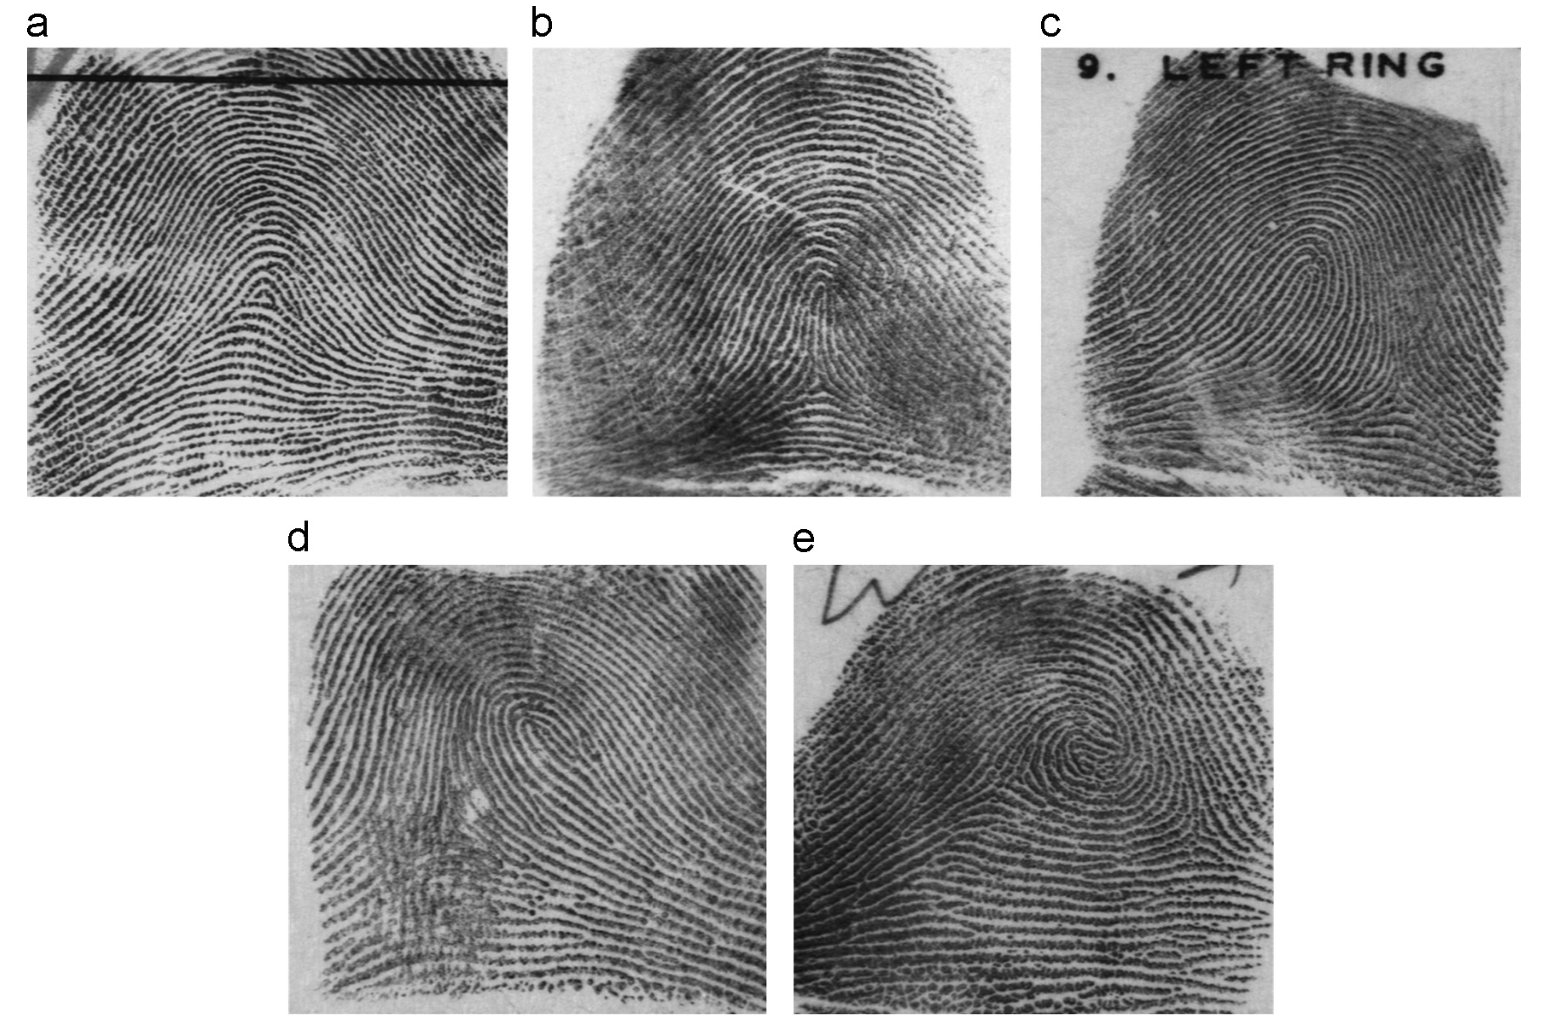
\includegraphics[width=8cm]{fig/Fingerprint_classes.png}
	\end{center}
	\caption{Examples of fingerprint classes: (a) Arch (b) Tented Arch (c) Left Loop (d) Right Loop  (e) Whorl \cite{cao2013fingerprint}} 
	\label{fig.fingerprint_classes}
\end{figure}




%-------------------------------------------------------------------------

%\section{Related Work}
%%!TEX root = main.tex

The milestone of the deep reinforcement learning is deep Q-learning(DQN)\cite{mnih2013playing}, a variant of Q-learning, proposed by DeepMind. It is the first deep learning model trying to learn control policies with reinforcement learning. In 2015, DeepMind presented an improved version of DQN\cite{mnih2015human}. Their work outperformed previous algorithms and achieved a capability comparable to that of professional human-being.
%

While DQN performs well in fully-observable environments, it achieves poor result in partially observable environments. To address this problem, Hausknecht and Stone \textit{et al.}~\cite{hausknecht2015deep} introduced the Deep Recurrent Q-Networks(DRQN). The idea is to build a recurrent neural network such as LSTM on top of the DQN model.
%

One drawback of DQN is that it needs to aggregate over time to overcome data non-stationarity. To reduce the overhead caused by experience replay, DeepMind \cite{mnih2016asynchronous} proposed a another paradigm for deep reinforcement learning: multiple agents are running in parallel asynchronously on multiple instances of the environment. Using the paradigm makes Q-learning both efficient and compatible with deep neural network at the same time. They named their best method \textit{asynchronous advantage actor-critic} (A3C). Experiments showed that A3C not only achieved better result but also required less computational cost.
%

%% Alpha go 
 More recently, AlphaGo\cite{brockman2016openai}, which is also developed by DeepMind, defeated Lee Sedol and became the first 'Artificial Intelligence' who beated 9-dan professional human Go player. Behind the AlphaGo is deep neutral network integrated with reinforcement learning improving the play strategy.


%% RDQN 
 RDQN sometimes learn unrealistically high action values because it includes a maximization step over estimated action values, which tends to
 prefer overestimated to underestimated values. This has been demonstrated in some games in the Atari 2600 domain. The idea of double Q-learning algorithm \cite{van2015deep} not only yields more accurate value estimates, but leads to much higher scores on several games. This demonstrates that the overestimations of DQN indeed lead to poorer policies and that it is beneficial to reduce them.


% liyang
% Other application of reinforcement Learning in designing game includes linear evaluation function-based learning of local shape in the game of Go \cite{silver2007reinforcement} and learning control policies for text-based games \cite{narasimhan2015language}

\section{Problem statement}

The challenge of classifying fingerprint includes: 
%
1) the quality of some fingerprints images are poor; 
%
2) the inter-class dissimilarity is small and the intra-class similarity is small; 
%
3) some fingerprints can be classified into multiple classes and there exists some ambiguity in the label.

To solve these problems, many researchers propose to use handcrafted features instead of raw fingerprint images for classification and many methods have been proposed, including ridge, orientation field, singular point.
%
Kai Cao \textit{et al.}\cite{cao2013fingerprint} propose to a novel method to extract fingerprint orientation feature and use a hierarchical classifier for classification.
%
Ruxin Wang \textit{et al.} \cite{wang2014fingerprint} also use orientation filed as feature. By adopting a stacked autoencoder , they achieve 93.1\% in four-class classification.
%

Using accurate handcrafted features can improve performance.  However, due to the existence of noise and poor image quality, the accuracy of handcrafted features cannot be guaranteed.
%
Convolutional neural network (CNN) has the capability of learning features and it can be directly applied on raw images. CNN also exhibits powerful classification capability in many areas.\cite{szegedy2016rethinking}.



%-------------------------------------------------------------------------

\section{Proposed research}
%!TEX root = main.tex

In this project, we aim to develop and implement a deep learning algorithm that takes a fingerprint image as an input and classify it into one of the five pattern class types of a) Arch; b) Tented Arch; c) Left Loop; d) Right Loop; or e) Whorl. 

\subsection{Feature Extraction}
%
We will first apply raw fingerprint images to train a CNN for classification. The outputs of some intermediate layer  of CNN will be used as features for possibly a support vector machine classifier.
%
We will consider using automated extracted features (\textit{e.g.},orientation filed) as inputs for CNN training, with the goal of combining raw images and automated features as input to train CNN.

For CNN architecture, we will first use canonical architecture ( such as 5 \textit{convolutional} + 3 \textit{fully-connected} in \textit{AlexNet}\cite{krizhevsky2012imagenet}). We will then modify the CNN architecture to improve the performance.
%
\subsection{Classifier}
%
We will consider two classifiers. The first one is the prediction layer of CNN. The values in last layer indicates the predicted probabilities of each class.
%
The second one is support vector machine (SVM whose input features comprise of the CNN’s middle or last layers.

\subsection{Data Augmentation}
%
To further improve the performance, we will use data augmentation technique to generate more training samples in order to increase the generalization ability of our model.



%-------------------------------------------------------------------------

\section{Dataset}

In this project, we will use NIST Special Database 4 \cite{nist-db-4} for our experiments. Some samples can be seen in Fig.\ref{fig.fingerprint_classes}.
%
The NIST database of fingerprint images contains 2000 8-bit gray scale fingerprint image pairs, totally 4000 images.
%
Each image is 512-by-512 pixels with 32 rows of white space at the bottom and classified using one of the five following classes: Arch, Left and Right Loops, Tented Arch, Whorl.
%
Each of the five classes has 400 pairs. Each of the fingerprint pairs are two completely different rollings of the same fingerprint.


%-------------------------------------------------------------------------




%-------------------------------------------------------------------------


{\small
\bibliographystyle{ieee}
\bibliography{egbib}
}

\end{document}
